\documentclass[DD.tex]{subfiles}
\begin{document}
\section{Architectural design}
\subsection{Overview: High-level}

The system is going to be implemented with a three tier architecture. Tiers are  as briefly described by the following schemas.

\begin{figure}[h!]
	\centering
	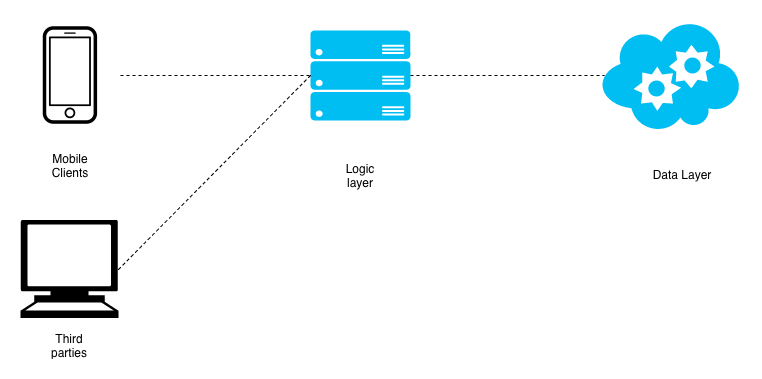
\includegraphics[height=6.00cm,keepaspectratio]{Figures/GeneralSchema}
	\caption{High level view of the system's architecture}
\end{figure}

The decision of this kind of architecture has been taken in order to build the system in the most modular possibile way. Here are described layer organisation:

\begin{itemize}
	\item Presentation layer:\begin{itemize}
			\item \textit{Mobile clients}: users will be given with a iOS application which will be a view of the entire system.
			\item \textit{Third parties}: third parties will be given with a light web interfaces to register/manage API access and they will be authorised to communicate with the system.
			\end{itemize}
	\item \textit{Logic layer}: logic layer will implement all the logic of the entire system and will handle communications between clients' app and the data layer.
	\item \textit{Data layer}: data layer will be implemented in third party's cloud system and will keep persistent users' data.
\end{itemize}

The idea is to keep as separate as possibile the logic layer from the data layer in order to let the system grow in a modular fashion and let us change cloud data provider as the system's dimension grow with the minimum effort.

\newpage
\begin{figure}[h!]
	\centering
	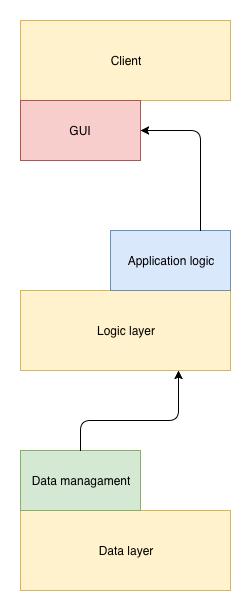
\includegraphics[height=8.00cm,keepaspectratio]{Figures/ThreeTierSchema}
	\caption{Distribution of application's function among the tier}
\end{figure}
\newpage

\subsection{Component view}
We now provide a high level view of system's components. The whole system can be seen as two main client component \textit{WebInterface} e \textit{Mobile Application} that consumes services offered by a set of logic components: \textit{HealthSharing manager}, \textit{SOS manager}, \textit{RunEvent Manager}, \textit{Access Manager}. Each of them, will be interfaced with the \textit{DatabaseLink Manager} which provides transparent access to the tier devoted to persistency.
\\ We are going to provide further details of each subsystem.

\begin{figure}[h!]
	\centering
	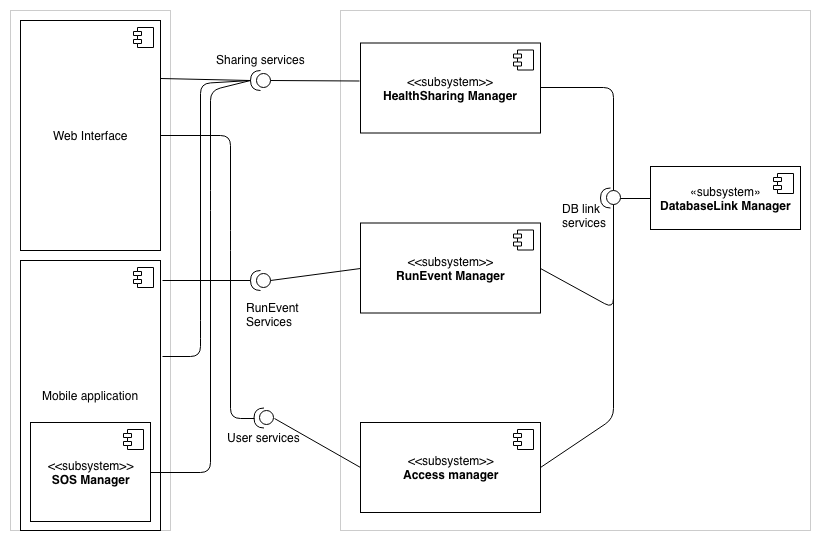
\includegraphics[height=8.00cm,keepaspectratio]{Figures/ComponentOverview}
	\caption{High level overview of system components.}
\end{figure}

\newpage
\subsubsection{Component view of HealthSharing Manager}
HealthSharing manager is composed of two main submodule: \begin{itemize}
	\item Access Policy Manager Module.
	\item Data Manager Module.
	\item Data elaboration Module.
\end{itemize}

The \textit{Access Policy Manager Module} works as a manager of all the policies associated with data sharing. It provides the list of active sharing to users and it let them manage active policies such as accepting new sharing request, or change/delete active policies. Moreover this component is also used by third parties that have to be able to subscribe to users data.\\
The \textit{Data Manager Module} has to handle all the operations of retrieving/storing data between users' app and databases. It also has to guarente data consistency in the whole system.
	\\
The \textit{Data Elaboration Module} has to handle all the operations devoted to make data anonymous and to handle request of aggregated data from third parties.

\begin{figure}[h!]
	\centering
	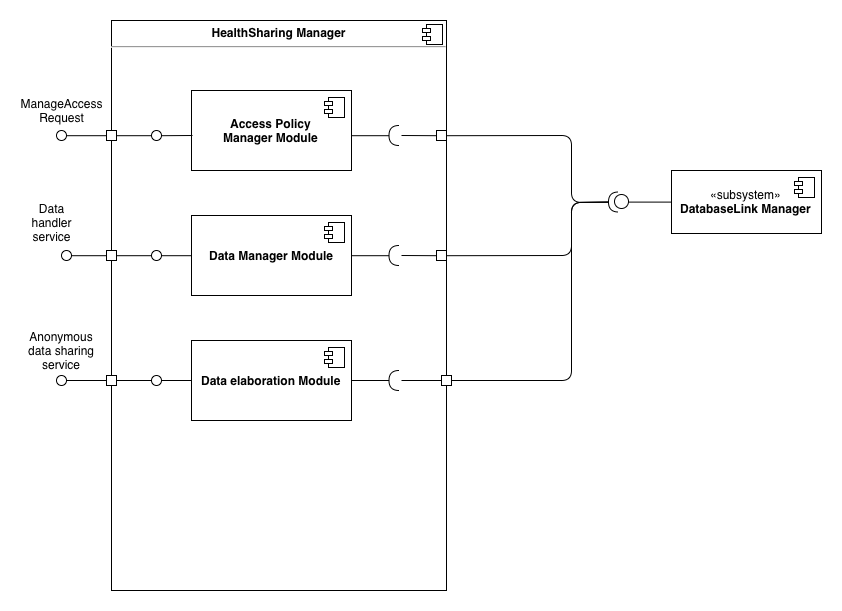
\includegraphics[height=8.00cm,keepaspectratio]{Figures/HealthSharingManagerComponent}
	\caption{Specific description for HealthSharing Manager component.}
\end{figure}
\newpage

\subsubsection{Component view of SOS Manager}
The \textit{Anomaly Detection Module} has to live read and control heartbeat data from users that have activated SOS functionality in their mobile application.
\begin{figure}[h!]
	\centering
	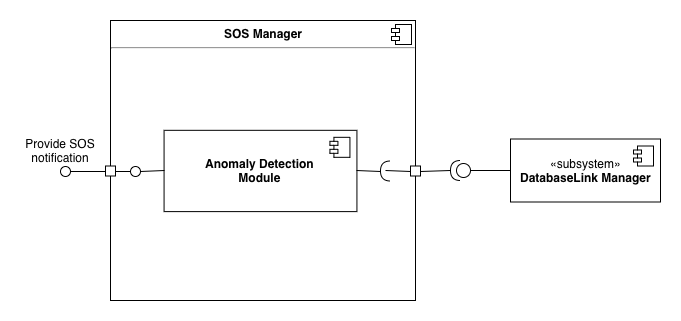
\includegraphics[height=6.00cm,keepaspectratio]{Figures/SOSManagerComponent}
	\caption{Specific description for HealthSharing Manager component.}
\end{figure}
\newpage


\subsubsection{Component view of RunEventManager}
\begin{figure}[h!]
	\centering
	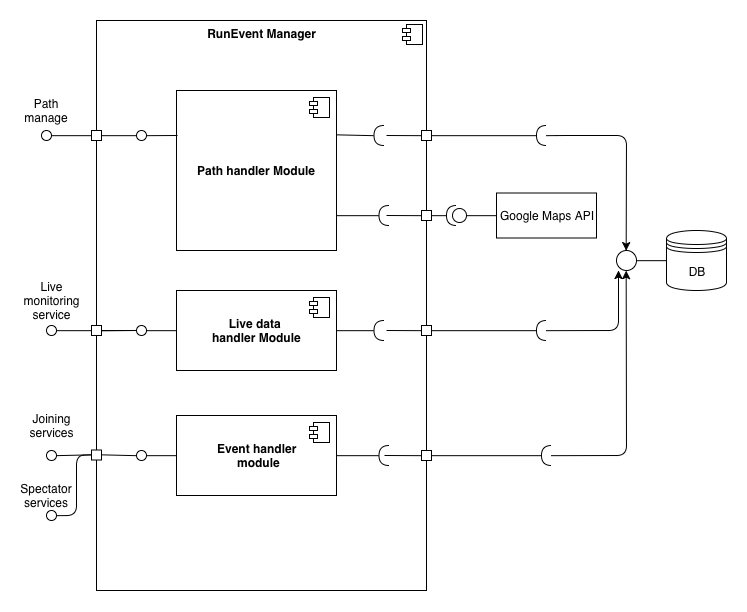
\includegraphics[height=10.00cm,keepaspectratio]{Figures/RunEventManagerComponent}
	\caption{Specific description for RunEvent manager.}
\end{figure}

RunEvent manager is composed of three main submodule: \begin{itemize}
	\item PathHandler module.
	\item Live data handler module.
	\item Event handler module.
\end{itemize}

The \textit{PathHandler module} has to offer services for creation and paths managing to users. In order to to that, it has to communicate with external Google Maps API.\\\\
The \textit{Live data handler module} has to handle incoming live data from users and prepare and aggregated versione for spectators. Moreover it has to make them persistent for future access.\\\\
The \textit{Event handler module} has to handle events creation, users' joining operations and spectators.

\newpage
\subsubsection{Component view of access manager}
\begin{figure}[h!]
	\centering
	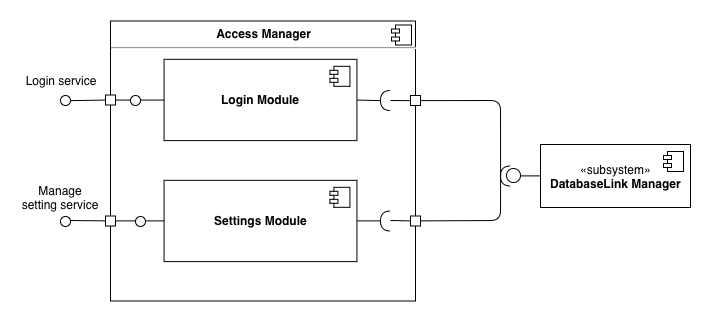
\includegraphics[height=7.00cm,keepaspectratio]{Figures/AccessManagerComponent}
	\caption{Specific description for Access Manager component.}
\end{figure}

Access Manager is composed of two main submodule: 
\begin{itemize}
	\item Login Module
	\item Setting Module
\end{itemize}

The \textit{Login Module} offers all the function devoted to login for both users and third parties.\\
The \textit{Setting Module} offers services devoted to let users to change and manage their preferences.



\newpage
\subsection{Deployment view}

\begin{figure}[h!]
	\centering
	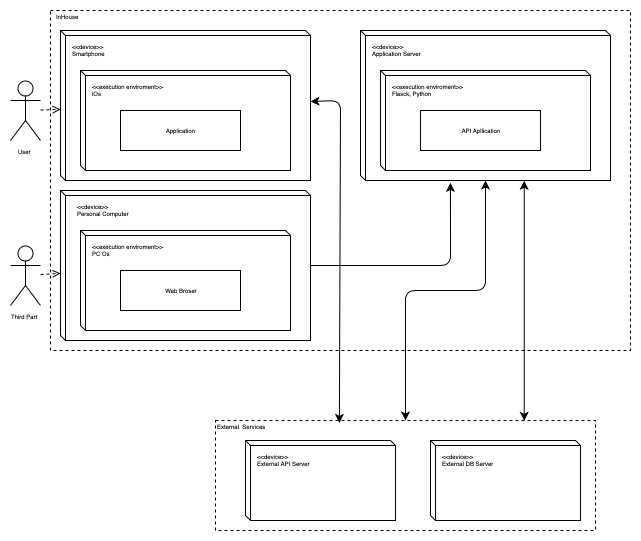
\includegraphics[height=10.00cm,keepaspectratio]{Figures/DeploymentDiagram}
	\caption{Deployment Dyagram}
\end{figure}

The Deployment diagram emphasises the nodes on which the platform runs:\\
\textbf{InHouse} box represent the components developed inside the company.
The components in the \textbf{External box} represent the “on demand” software.\\
\begin{itemize}
\item	\textbf{Smartphone} : the application deployed on the iOs Smartphone used by the user. Users are able to retrieve data from the application server and, also, from the external 			server API directly (e.g. maps by Google Maps)
\item \textbf{Web Browser API Interface} : A web page for Third Parties registration. It provides a secret to do a request to the API Server.
\item \textbf{Application Server }: the  main logic core of the application. It’s the only one access point to the DB but also it communicates with the external server API
\item  \textbf{External Service} : Both the external services are represented as a blackbox because we don’t know how they are implemented.
\end{itemize}
\newpage


\subsection{Runtime view}
\newpage
\subsection{Component interfaces}
\begin{figure}[!th]
	\centering
	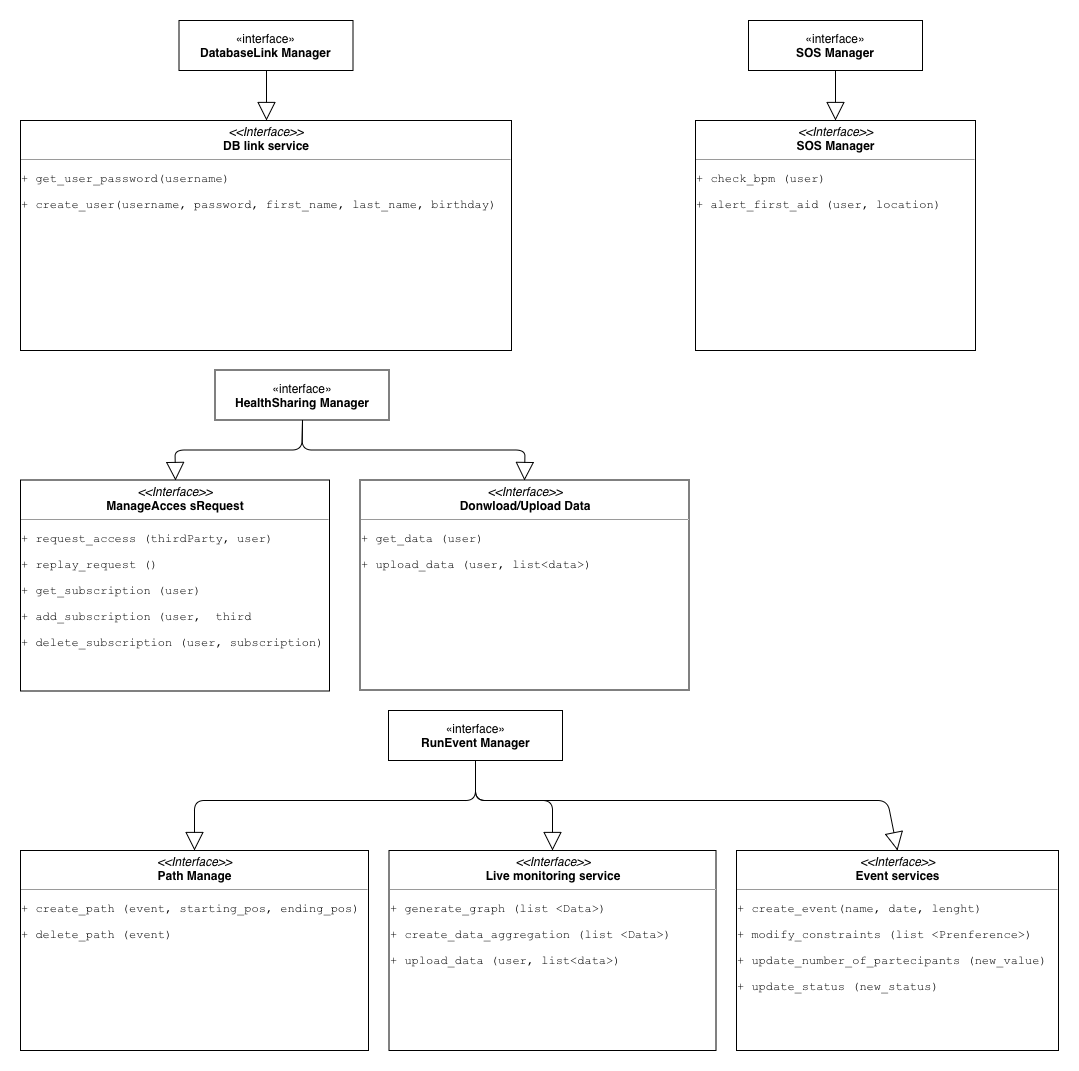
\includegraphics[height=16.00cm,keepaspectratio]{Figures/Interfaces}
	\caption{Components' interfaces descriptions diagram}
\end{figure}

\newpage

\subsubsection{API structure}
The whole TrackMe infrastructure will be connected trough a RESTful API system. JSON will be used as serialisation data format.\\
All the api system will be implemented referring to a single endpoint www.data4help.cloud that TrackMe will buy for the implementation of this project.
\\Users' applications and third parties will refer to different subdomain:

\begin{itemize}
	\item \textit{\textbf{www.data4help.cloud/api/users}}: it will be the specific endpoint for the application that serves users.
	\item \textit{\textbf{www.data4help.cloud/api/thirdparties}}: it will be the specific endpoint for thirdparties.
\end{itemize}

Here a complete description of each supported methods follows:

\begin{itemize}
	\item method 1:
	\item method 2:
\end{itemize}

\newpage
\subsection{Selected architectural styles and patterns}
Data4Help system is based on a tree tier architecture:
\subsubsection{Overall Description}
\begin{itemize}
	\item \textbf{Presentation Tier} has to present the data to the user in such a way that they are meaningful for the user’s perspective. It displays information to the user obtained communicating with the other two tiers. For example, if a user performs a tap on the button “create a new run event” the communication tier send a query to the Logic Tier that answers with a message requiring for information to create an Event and so on.
		To be quick to react in case of “Anomaly detection”, instead of putting the logic of continuous checking of the vital parameters into the Logic Tiers (as the entire logic of the application) the Presentation Tier (the application) contains also this component. Doing this we will be able to speedy react and call the ambulance in the shortest way possible. We are also able to react in narrow situation as absence of field coperture or not working internet network.
	\item \textbf{Logic Tier} has the entire logic needed for the application (excluding the “Anomaly detection” component as described above). It receives the requests from the Presentation Tier and, if needed, queries the Data tier before then sending the reply.
	\item \textbf{Data Tier} is composed of a DBMS that provide an interface to the DataBase externally located. It contains all the data in a Relational Schema (ER) (view fig XXX)\\\\
	The separation between the different layers allow us to upgrade or replace a single tier without affecting the others
\end{itemize}
\subsubsection{Design Patterns}

\begin{itemize}
	\item \textbf{Model View Controller (MVC)}\\
		\textbf{MVC in a nutshell}\\
		The MVC is a pattern that describe how to separate the components of the project in such a way to maintain high level of separation. \\
		\vspace{-5mm}
		\begin{itemize}
		\setlength\itemsep{-0.9em}
			\item\textbf{Model} is the section that contains only the data of the application\\
			\item\textbf{View} is the section that contains the component needed to represent information\\
			\item\textbf{Controller} is the section that contains the logic of the application\\
		\end{itemize}
		\textbf{MVC in Data4Help}\\
		In Data4Help the \textbf{Model} is the persistent data storage with the Entity-Relation SQL Database (view section 2.6.1) placed externally.\\
		The \textbf{View} is the application displayed on the smartphone, is the only point of interaction with the client.
		This component contains the "UI Controller" that is the logic to handle the tap on the UI. It also contains the logic of AutomatedSOS because is required to be very reactive in case of emergency \\
		The \textbf{Controller} is placed on the web server and is accessible as a RESTful endpoint. It contains the logic of the application \\
		\item \textbf{Altri pattern??}\\
\end{itemize}

\subsubsection{Other design decision}

\begin{itemize}
	\item We decided not to let logic components to directly deal with the database but to interleave the \textit{Database Link Manager} in order to build the logic layer independently from the persistency layer. Developers will be able to change the way the system interacts with the database or to change database's interfaces without having to change all the components. 
\end{itemize}
\end{document}